

\section{EVALUATION}
This section presents the experimental results by measuring the performance of Peapods. The experimental machine has an Intel Core i7-4770S quad-core processor running a Linux operating system (kernel version 3.13.1).We experimented with the PolarSSL cryptographic algorithm library and used Peapods to protect 2048-bit RSA private key calculations after splitting into 128 transactions and 256 transactions.The comparison objects in the experiment include: (1) the official default configuration of PolarSSL (version 1.3.9), (2) Peapods\_128, the Peapods split into 128 transactions,(3) Peapods\_256, the Peapods split into 256 transactions.
\subsection{Local Performance}
The local throughput for PolarSSL, Peapods\_128, and Peapods\_256 are: 391/s, 341/s, and 352/s (4 threads).Compared to PolarSSL, the performance of Peapods\_128 and Peapods\_256 dropped by 12.8\% and 10.0\%, respectively.The performance overhead introduced by Peapods mainly comes from: (1) waste of CPU clock cycles due to rollback of transactions; (2) encryption and decryption protection of sensitive information and intermediate calculation results; (3) preloading.The reason Peapods\_256 performs slightly better than Peapods\_128 is that the more granular splitting reduces transaction abort due to time-outs and other factors.

\begin{figure*}[!htb]
\centering
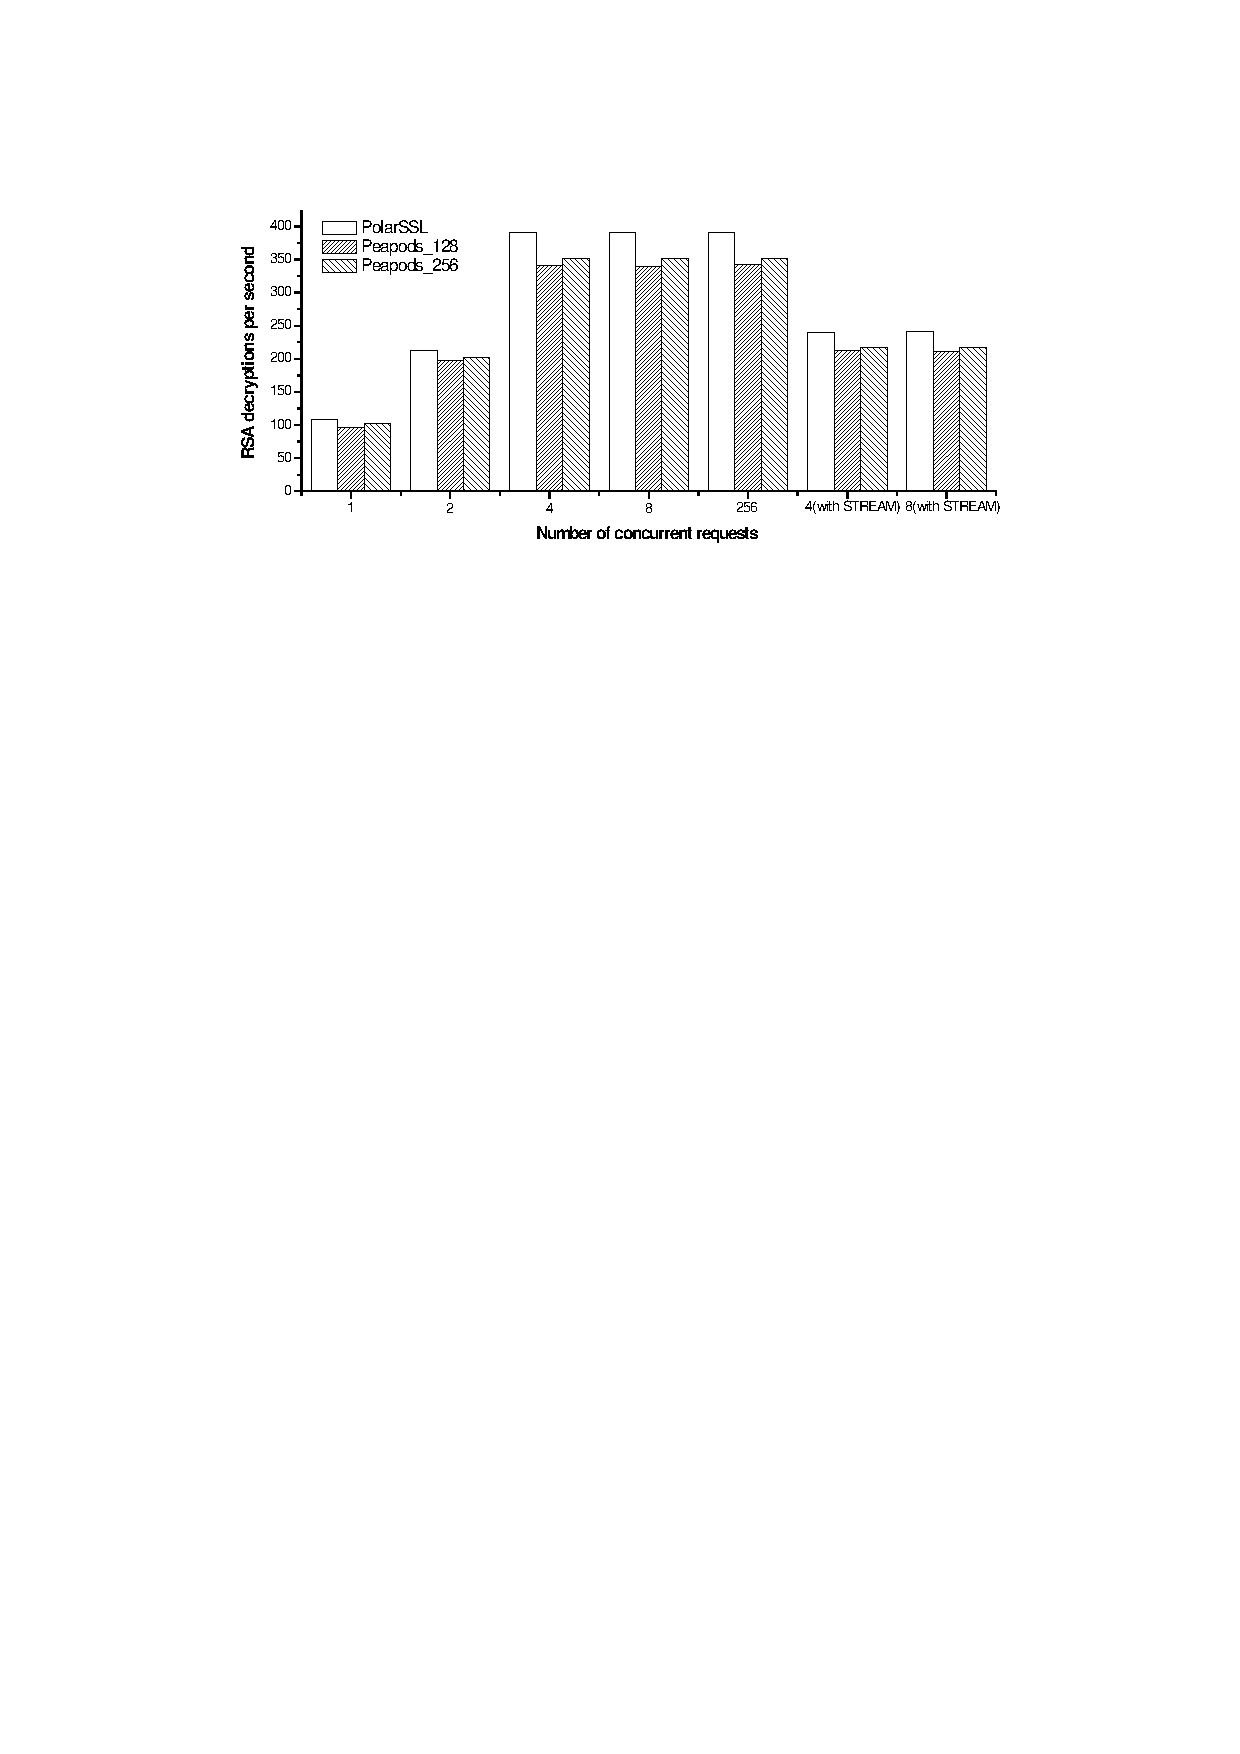
\includegraphics[width=0.9\textwidth]{rsa_local_peapods.pdf}
\caption{Local Performance}
\label{fig:rsa_local_peapods}
\end{figure*}

During the sensitive information calculation phase, Peapods relies on Intel TSX to ensure the confidentiality of protected sensitive information. However, cache(the foundation of TSX implementation) is limited by space and shared by all cores. This might lead to denial of service(DoS) attacks.Most of Intel's CPUs implement 8-way group-associated L1D caches, so 9 memory accesses to the same set of caches will inevitably result in transaction termination.Moreover, Intel does not guarantee that all L1D caches can be used in TSX.In addition, a memory-intensive process may also make it difficult for Peapods to complete a transaction.Due to the shared L3 cache, it is likely to evict the cache line that Peapods is using.Users can use T-SPLIT function to split the sensitive information calculation process, reducing the execution time and memory usage of a single transaction, which can effectively alleviate the impact of DoS attacks on Peapods.We completed the experiment to verify this result.

We measured whether a memory-intensive program will have a greater impact on Peapods by running the Geekbench 3 memory stress test while Peapods is performing RSA private key calculations.In the experiment, 4 different memory stress tests will run on all CPU cores, which will cause about 10GB/s of memory data transfer.The maximum memory transfer rate supported by the machine when no user program is running is 13.7GB/s.Peapods\_128 dropped from 341 RSA decryptions per second to 212 RSA decryptions per second, performance decreased by 37.8\%, Peapods\_256 decreased from 352 RSA decryptions per second to 218 RSA decryptions per second, performance decreased by 38.1\%.PolarSSL decreased from 391 RSA decryptions per second to 241 RSA decryptions per second, performance decreased by 38.4\%.

In short, the performance overhead of Peapods is acceptable. At the same time, Peapods perform better than other transaction-based protection due to preloaded optimizations.

\subsection{Factors affecting transaction abort}
We also evaluated the impact of fine-grained sensitive computational process splitting on transaction abort. We use peapods to protect a simple program that is set to a transaction area after processing, then constantly adjust the memory usage and transaction time in the transaction through write operations and loop instructions. We measured the duration of each
transaction by instrumenting the source code that begins and ends transactions with rdtsc instructions.Table \ref{tab:factors_abort_1} and Table \ref{tab:factors_abort_4} display the effect of transaction time and memory usage on transaction abort.For each transaction, we conducted 200 experiments, the data(abort rate) in the table is the average of the experimental results.
\begin{table}[htbp]
 \caption{\label{tab:factors_abort_1} Effect of transaction time and memory usage on transaction abort(single thread)}
 \centering
 \begin{tabular}{|c|c|c|c|c|c|}
  \hline
  \diagbox{\textbf{Memory(bytes)}}{\textbf{Time(cycles)}} & 3000 & 30000 & 120000 & 210000 & 300000 \\
  \hline
  0 & 0 & 1.14\% & 3.92\% & 6.94\% & 8.23\% \\
  \hline
  300 & 0.54\% & 1.35\% & 4.42\% & 7.36\% & 8.85\% \\
  \hline
  1200 & 0.64\% & 1.72\% & 4.69\% & 7.26\% & 9.72\% \\
  \hline
  2100 & 0.68\% & 2.03\% & 4.91\% & 8.18\% & 10.25\% \\
  \hline
  3000 & 0.68\% & 2.18\% & 5.23\% & 8.42\% & 11.45\% \\
  \hline
 \end{tabular}
\end{table}

\begin{table}[htbp]
 \caption{\label{tab:factors_abort_4} Effect of transaction time and memory usage on transaction abort(4 threads)}
 \centering
 \begin{tabular}{|c|c|c|c|c|c|}
  \hline
  \diagbox{\textbf{Memory(bytes)}}{\textbf{Time(cycles)}} & 3000 & 30000 & 120000 & 210000 & 300000 \\
  \hline
  0 & 0 & 1.62\% & 5.12\% & 8.96\% & 12.23\% \\
  \hline
  300 & 0.76\% & 2.17\% & 6.37\% & 9.43\% & 12.34\% \\
  \hline
  1200 & 1.14\% & 2.93\% & 7.67\% & 10.3\% & 14.63\% \\
  \hline
  2100 & 0.98\% & 2.93\% & 8.46\% & 13.64\% & 17.35\% \\
  \hline
  3000 & 1.28\% & 3.88\% & 9.76\% & 14.92\% & 18.05\% \\
  \hline
 \end{tabular}
\end{table}

It is not difficult to find that transaction time and memory usage have an impact on the transaction abort.The impact of transaction time on transaction abort is very intuitive. As the transaction time increases, the transaction abort rate increases greatly.When the memory usage is small, the change in memory usage has a greater impact on the transaction abort. As the memory usage increases, this effect is gradually reduced.When the memory usage increases to a certain value, the transaction abort rate increases rapidly (not shown in the tables), which is caused by the cache capacity limit.

%abort�ʵ�ͼ
\subsection{Impact on Concurrent Processes}
We used Geekbench 3 to test Peapods' impact on other concurrent processes.Figure X shows Geekbench 3 scores in multi-core mode and single-core mode.The baseline is a score in clean environment.

The Geekbench 3 benchmark program performed integer, floating point, and memory bandwidth tests, respectively.PolarSSL, Peapods\_128, and Peapods\_256 experiments have similar scores. Unprotected PolarSSL is slightly better than Peapods.When Geekbench occupies multiple cores, the load change that simultaneously processes RSA private key calculation requests cannot be ignored��the baseline has a clear demarcation from other scores.It is worth noting that XMM registers are mainly used for floating-point calculations, and generally only 1-2 XMM registers are used.When the environment has only a small number of floating point calculations, we will not significantly affect the XMM7 register from the register allocation pool. When there are a large number of floating point calculations in the environment, the overall performance will be slightly reduced.In short, Peapods do not have a significant additional impact on other concurrent processes.

\begin{figure*}[!htb]
\centering
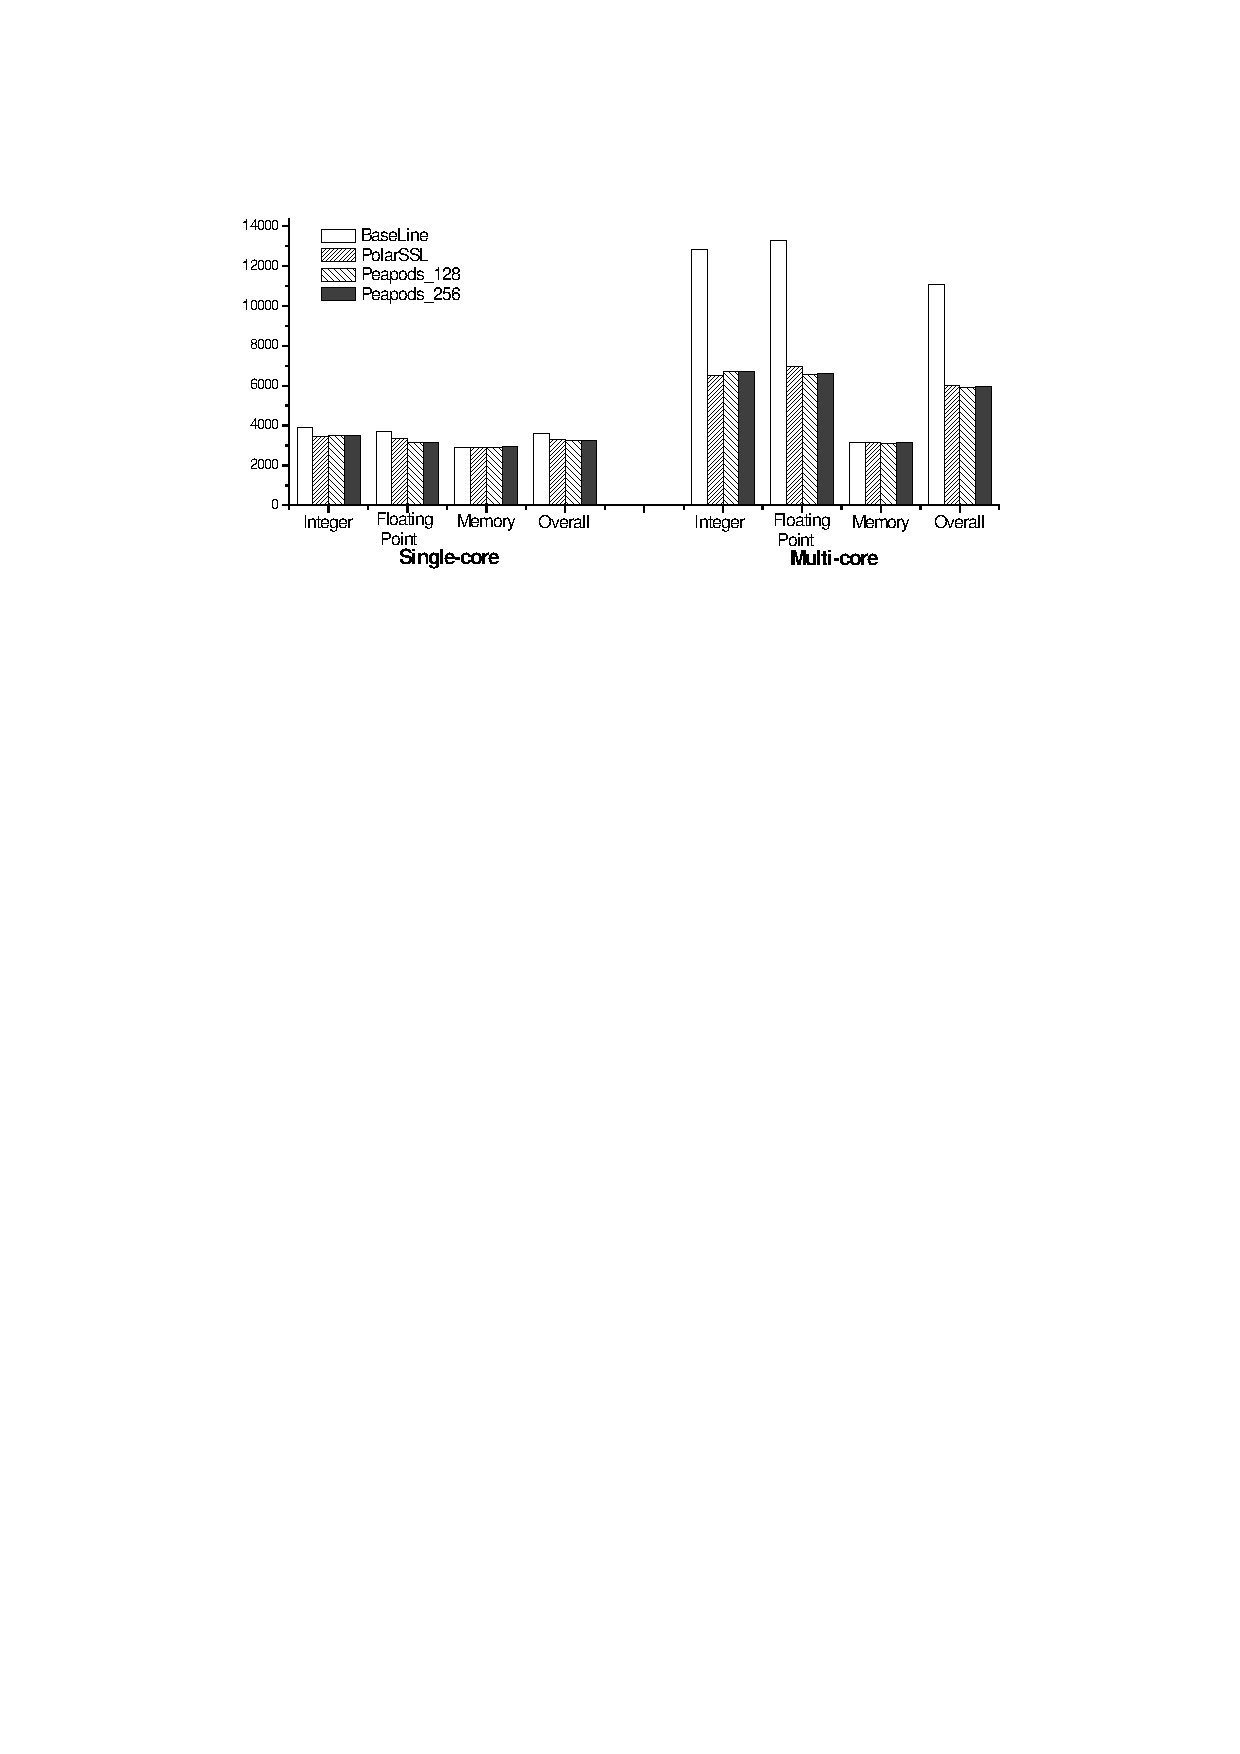
\includegraphics[width=0.9\textwidth]{stream.pdf}
\caption{Impact on Concurrent Processes}
\label{fig:stream}
\end{figure*}
\subsection{��SGX�ıȽ�}

